\chapter{Controlador de corriente} \chapterlabel{Informe/4-ControladorCorriente} \label{cap:ControladorCorriente}

En este capítulo se diseña y modela el circuito encargado de controlar la corriente que circula por el electroimán. Como se vio en el capítulo anterior, el sistema trabaja con corrientes elevadas por lo que se implementan estrategias de conmutación para reducir las pérdidas de energía. Para ello se utiliza una topología de puente H con cuatro MOSFET y un \textsl{driver} que los controla. Además, se detallan los criterios tenidos en cuenta al momento de  elegir  y dimensionar todos los componentes que intervienen para lograr el correcto funcionamiento del controlador de corriente. Por último, se obtiene su función transferencia  para ser utilizada en el diseño del compensador.

\section{Descripción general}\label{sec_descripcion-general}

\colorbox{red}{Creo que estaría buena una intro para mas contexto de qué función cumple}

Como se describió en el capítulo \ref{cap:Introducción}, el dispositivo completo se trata de un sistema realimentado en el que el control de la posición se realiza regulando la corriente del electroimán según lo requiera el compensador (tanto analógico, como digital). Si bien aún no se aborda el diseño de este bloque compensador, se sabe (o se desea) que su salida será en forma de tensión, con niveles entre $0\:V$ y $5\:V$. Por otro lado, el electroimán requiere corrientes de hasta como $30\:A$. Por lo tanto es necesario diseñar un controlador (o \textsl{driver}) de corriente que sea capaz de entregar la corriente requerida, y que esta sea controlada por una tensión de entrada(tensión de referencia).

Como se analizó en el capitulo \ref{cap:CaracterizacionElectroiman}, en la sección ASDASDAS se llega a la ecuación \ref{eq_fuerza_magnetica}, que se repite a continuación. 

\begin{equation*}
	\abs{F_{m}}=\frac{i^{2}*N^{2}*\mu_{o}*A}{4*Y_{g}^{2}}
\end{equation*}

En ella se ve que la fuerza magnética depende de la corriente del bobinado. Por lo tanto si se desea regular la fuerza electromagnética, esto se puede lograr a partir de modificar la intensidad de corriente.

\colorbox{red}{esto estaba antes}Esto se logra modificando la intensidad de la corriente que circula por su bobinado como lo indica la expresión \ref{eq_fuerza_magnetica}. Por lo tanto, es necesario diseñar una fuente de alimentación que sea capaz de proveer la corriente requerida. 

\subsection{Comportamiento eléctrico del electroimán}

Como se analizó en el capítulo \ref{cap:CaracterizacionElectroiman}, el electroimán puede ser modelado como una inductancia que varía con la distancia de entrehierro ($Y_g$) y una resistencia serie ($R_L$) correspondiente al bobinado. Es decir, como un circuito RL serie cuya relación entre corriente de salida y tensión de entrada (admitancia) se muestra en la expresión \ref{eq_corriente}.

\begin{equation} \label{eq_corriente}
\frac{I_L}{V_L}(s)=\frac{1}{s*L_{(Y_g)}+R_L}
\end{equation}

Al aplicar la transformada inversa de Laplace a la expresión  \ref{eq_corriente}, se obtiene la respuesta temporal de la corriente ante un escalón de tensión con amplitud $v_L$ en la entrada, considerando corriente inicial $I_o$ y constante de tiempo $\tau=\frac{L_{(Y_g)}}{R_L}$.

\begin{equation} \label{eq_corriente_temporal_cond_iniciales}
	i_L(t)=\frac{v_L}{R_L} + (I_o-\frac{v_L}{R_L})*e^{-\frac{t}{\tau}}
\end{equation}

En la expresión \ref{eq_corriente_temporal_cond_iniciales} se puede observar que la respuesta al escalón está compuesta por dos partes: un término con una exponencial negativa correspondiente al transitorio, y un término constante correspondiente al valor en régimen permanente $\frac{v_L}{R_L}$. El primero es el responsable de que la corriente en el inductor crezca de manera amortiguada, hasta alcanzar el valor de régimen permanente luego de cierto tiempo. Este comportamiento se puede observar en la simulación realizada en la figura \ref{fig:img_respuesta_escalon}. En la parte superior se observa la tensión de entrada y, en la inferior, la corriente del electroimán. Este análisis resulta de utilidad para conocer el comportamiento del electroimán y diseñar un controlador de corriente adecuado.


\begin{figure}[H]
	\centering
	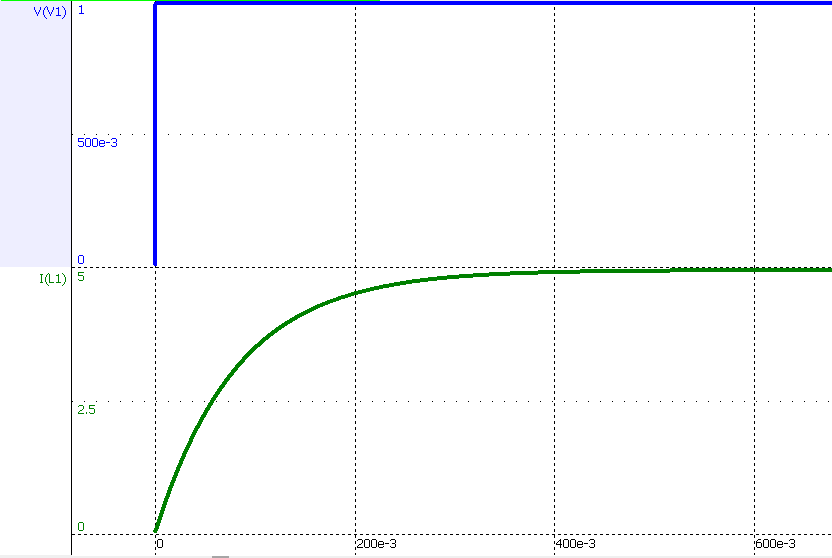
\includegraphics[scale=0.5]{corriente_escalon.png}
	\caption{Respuesta ante una entrada en escalón.}
	\label{fig:img_respuesta_escalon}
\end{figure}


\section{Diseño del controlador}


Se desea controlar el valor medio de corriente que circula por el electroimán a partir de un sistema realimentado. Para ello se propone utilizar un controlador que trabaja en conmutación, alternando la alimentación del electroimán entre un valor superior positivo $\ V_{sup}$, y un valor inferior negativo $V_{inf}$. De esta manera, al controlar los tiempos de conmutación, se puede lograr una forma de onda como la que se muestra en la figura  \ref{fig:img_corriente_exponencial}. El resultado que se obtiene es una forma de onda con un valor medio correspondiente al deseado y un ripple superpuesto. La idea es que este ripple sea pequeño comparado con el valor medio, de manera que la planta pueda filtrarlo. 

\begin{figure}[H]
	\centering
	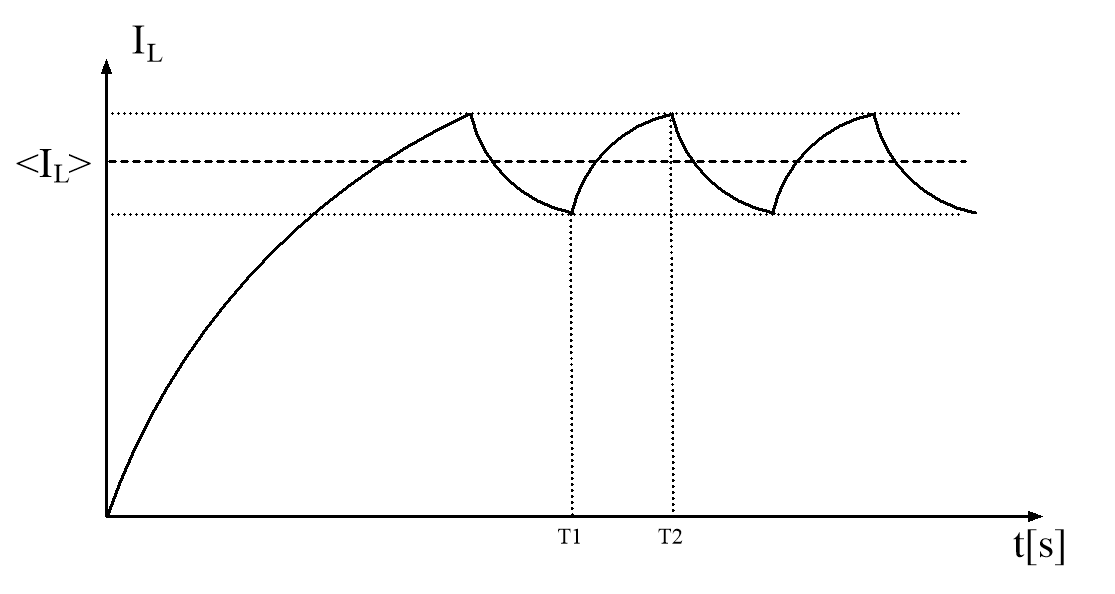
\includegraphics[scale=0.5]{Forma-de-onda-corriente-exponencial.png}
	\caption{Forma de onda de corriente y tensión en el electroimán.}
	\label{fig:img_corriente_exponencial}
\end{figure}

\colorbox{red}{modificar valores de imagen}

Si se elige un período de conmutación lo suficientemente chico con respecto a la constante de tiempo de la planta, la forma de onda de la corriente en estado estacionario puede ser aproximada a una onda triangular como se muestra en la figura \ref{fig:img_corriente_lineal}.

\begin{figure}[H]
	\centering
	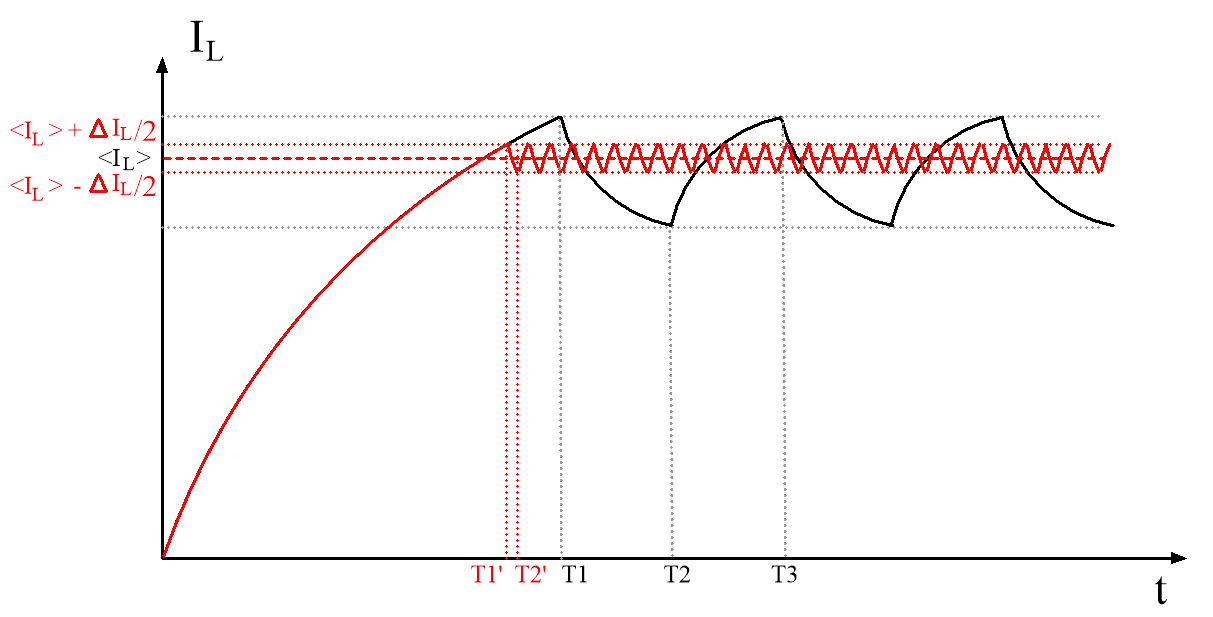
\includegraphics[scale=0.5]{Forma-de-onda-corriente-lineal.png}
	\caption{Forma de onda de corriente al disminuir el período de conmutación.}
	\label{fig:img_corriente_lineal}
\end{figure}

Se puede obtener una expresión lineal para cada tramo de la corriente triangular a partir de la serie de Taylor hasta el término de orden 1 de la ecuación \ref{eq_corriente_temporal_cond_iniciales}:

\begin{equation} \label{eq_corriente_taylor}
	i_L(t)=I_o -  (I_o-\frac{v_L}{R_L})*\frac{t}{\tau}
\end{equation}

Considerando el caso en que $I_o=0$ y  $\tau=\frac{L}{R_L}$ la expresión queda:

\begin{equation} \label{eq_corriente_taylor_2}
	i_L(t)= \frac{v_L}{L}*t
\end{equation}

\subsubsection{Análisis de estimación}

Como se menciono en la seccion INTRODUCCION para que la placa de control pueda mantener la distancia de separación $Y_{g}$ es necesario conocer su valor para luego actuar en consecuencia. Si bien se podrían utilizar sensores especializados para ello, para este proyecto se optó por medirla de manera indirecta a partir de la pendiente de la corriente que circula por el electroimán. De esta forma, se logran aplicar conceptos de estimación de variables, aprendidos durante la carrera.

Dado que existe una relación entre la inductancia del electroimán y la distancia de separación, es posible estimar esta última a partir de la forma de onda triangular de su corriente. Como se vio en el capítulo \ref{cap:ControladorCorriente}, el circuito equivalente del electroimán es del tipo RL serie. Por lo tanto, al conmutar la polaridad del inductor a una frecuencia mayor que su ancho de banda, se logra que la corriente crezca y decrezca de manera aproximadamente lineal (sin llegar a verse la forma exponencial). Por lo tanto, se puede extraer información del valor de la inductancia conociendo el valor de dichas pendientes

A partir de la ecuación de la corriente 3.4 si se aplica la derivada temporal se obtiene:

\begin{equation} \label{eq_corriente_taylor_2}
	\frac{di_L(t)}{dt}= \frac{v_L}{L}
\end{equation}


Como se vió en el capítulo 2, la inductancia es inversamente proporcional a la distancia de entrehierro, por lo tanto resulta:

\begin{equation} \label{eq_corriente_taylor_2}
	\frac{di_L(t)}{dt}= v_L*f(Y_g)
\end{equation}

Utilizando la expresión \ref{eq_inductancia_vs_y}, se llega a:

\begin{equation} \label{eq_corriente_taylor_2}
	\frac{di_L(t)}{dt}= Y_g*\frac{2}{N^2*A*\mu_o}*v_L
\end{equation}

Mirando la imagen 3.3 se puede plantear dos casos para la pendiente: la de subida, cuando $v_L=V_{sup}$ y la de bajada cuando $v_L=V_{inf}$ se obtienen dos expresiones para la pendiente:

\begin{equation} \label{eq_corriente_taylor_2}
	\frac{di_L(t)}{dt}_{sup}= Y_g*\frac{2}{N^2*A*\mu_o}*V_{sup}
\end{equation}


\begin{equation} \label{eq_corriente_taylor_2}
	\frac{di_L(t)}{dt}_{inf}= Y_g*\frac{2}{N^2*A*\mu_o}*V_{inf}
\end{equation}

Por lo tanto, si se elige que $|V_{sup}|=|V_{inf}|=|V_{cc}|$, la pendiente depende únicamente de la distancia $Y_g$ como se muestra en la ecuación de XD:

\begin{equation} \label{eq_corriente_taylor_2}
	\frac{di_L(t)}{dt}= Y_g*\frac{2}{N^2*A*\mu_o}*V_{cc}
\end{equation}

Este análisis resulta de interés ya que se puede observar que la pendiente tiene información de la distancia de entrehierro. Por lo tanto, se podría aplicar un estimador de posición a partir de medir la pendiente.

 %se podría aprovechar esa relación para aplicar estimación de variables y obtener, de manera indirecta un valor de distancia de entrehierro a partir de la pendiente de la corriente de la onda de corriente conmutada.

%Como se mencionó en la descripción general del dispositivo, es de interés realizar una estimación de la distancia del entrehierro a partir de la corriente que circular en el electroimán. Por este motivo es conveniente aprovechar la relación que existe entre la pendiente de la onda triangular, con la inductancia, que es inversamente propocional a la distancia de entrehierro.... De esta manera se puede implementar un circuito de estimación que trabaje a partir de medir la pendiente... Paroa que este circuito funcione correctamente, se debe respetar dos condiciones:

%*Que la magnitud de la pendiente solo sea sensible a la distancia de separación, y que todo lo demás sea constante (v_L)...

%*Que la pendiente en la subida sea igual en valor absoluto a la de bajada.  PAra que se pueda obtener un valor de posición en todo momento, sin que el sistema quede a lazo abierto

%*Que la estimación nunca se vea interrumpida, ya que el sisema quedaría a lazo abierto.
\subsection{Diseño del lazo de control de corriente}

%Como se mencionó previamente, para el diseño de la fuente de alimentación del electroimán se utilizará una topología de puente H trabajando en conmutación. Por lo tanto, para obtener el valor medio de corriente deseado es necesario controlar el tiempo que se le aplica cierta polaridad de tensión al electroimán. 

Como solución se propone un diagrama en bloques que se muestra en la figura XD. En este diagrama se realimenta la corriente y se compara con una corriente de referencia como Ie. Esta variable ingresa a un bloque -omparador con histéresis. 

El cual permite definir un margen de corriente $\Delta I_L$ de forma tal que, si la corriente que circula por el electroimán supera a la de referencia, no se producirá un cambio de polaridad en la tensión aplicada hasta que la supere por $\frac{\Delta I_L}{2}$. Análogamente, cuando comienza a decrecer, seguirá haciéndolo hasta que sea menor a la corriente de referencia menos $\frac{\Delta I_L}{2}$.

La forma de onda de corriente resultante se puede observar en la figura \ref{fig:img_corriente_exponencial-hist}.

\begin{figure}[H]
	\centering
	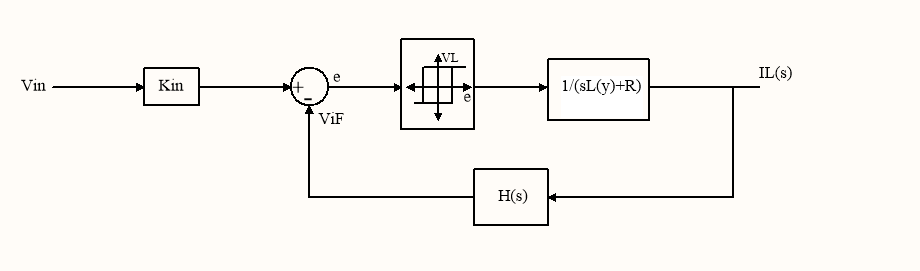
\includegraphics[width=\textwidth]{Diagrama-en-bloques.png}
	\caption{Diagrama en bloques del controlador de corriente con histéresis.}
	\label{fig:img_diag-en-bloques}
\end{figure}

Al analizar el diagrama en bloques planteado en la figura \ref{fig:img_diag-en-bloques-comparador-sin-hist} es posible notar que, una vez que la corriente del electroimán ($I_{L}(s)$) supere infinitesimalmente a la referencia, se producirá una conmutación en la polaridad de tensión aplicada al electroimán. Lo mismo sucede cuando es infinitesimalmente menor. El inconveniente que esto presenta es que se producirían conmutaciones extremadamente rápidas en torno al valor medio, por lo que sería necesario tener alta velocidad en conmutación. Por lo tanto, para reducir la frecuencia de esas oscilaciones, se propone agregar histéresis al controlador como se muestra en la figura \ref{fig:img_diag-en-bloques}.

Debido a que lo único que cambia es la polaridad de la tensión con la que se excita al electroimán, la constante de tiempo del circuito no cambia. Esto da como resultado que la corriente oscile sobre un valor medio con igual tiempo de crecimiento que de decrecimiento. Esta oscilación también es conocida como \textsl{ripple}. Su amplitud es fija y está determinada por el ancho de histéresis con el que se diseñe el controlador.


\subsection{Medición de corriente}


Como se puede ver en el diagrama en bloques \ref{fig:img_diag-en-bloques}, para poder realizar el control es necesario medir la corriente que circula por el electroimán y actuar en consecuencia.


Para hacer esto se debe utilizar un sensor que permita una medición de corriente hasta, por lo menos, $30\:A$  y con un error máximo tolerable tal que permita actuar al comparador y no afecte al sistema.

Los sensores de corriente trabajan en transresistencia, por lo tanto, se agrega el bloque H en el lazo de realimentación figura \ref{fig:img_diag-en-bloques-conH-y-Kin}. Ahora $V_{iL}=i_{L}*rm$. De esta forma ahora se está trabajando con tensiones por lo tanto la corriente de referencia se afecta por el bloque $K_{in}$ para obtener su equivalente en tensión. El bloque resultante es el siguiente:

\begin{figure}[H]
	\centering
	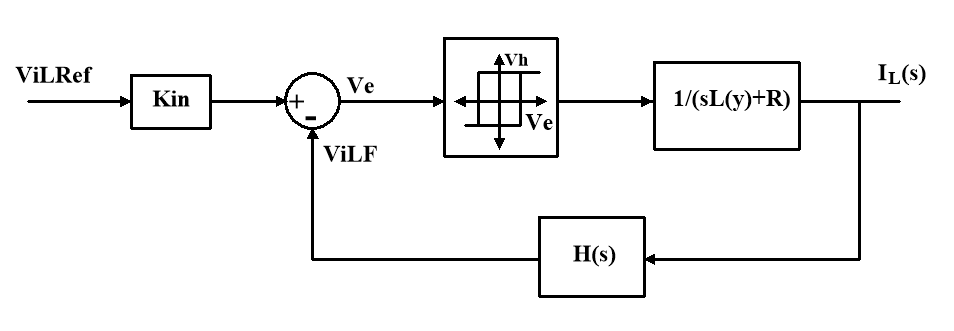
\includegraphics[width=\textwidth]{Diagrama-en-bloques-conH-y-Kin.png}
	\caption{Diagrama en bloques del controlador de corriente completo.}
	\label{fig:img_diag-en-bloques-conH-y-Kin}
\end{figure}

Se puede expresar al error que introduce el sensor de efecto hall como $V_{errSensor}$. Entonces la expresion de error $V_{e}$ resulta: 

\begin{equation}\label{eq_error_ve}
	V_{e}= K_{in}*I_{ref}-H*iL\pm V_{errSensor}=\triangle I \pm V_{errSensor}
\end{equation}


De esta forma, tomando el  caso extremo $K_{in}*I_{ref}=H*i_{L}$ el error obtenido $V_{e}=\pm V_{errSensor}$.
Es decir que el error es el propio error del sensor. Si se toma un ancho de histéresis mucho mayor al error máximo introducido por el sensor, este error no afectaría al sistema ya que seria despreciable a comparación del valor que deltaI debería alcanzar para que el comparador cambie de estado.

El error que introduce el sensor de efecto hall $V_{errSensor}$ debe ser mucho menor al ancho de histéresis del comparador.

\section{Elección y calculo de parámetros del controlador}
En esta sección se determinarán los parámetros críticos para el correcto funcionamiento del controlador de corriente.
\subsection{Cálculo de tensión de alimentación}
\colorbox{red}{Comenzar el diseño circuital? mm..}
Para comenzar el diseño circuital es importante determinar cómo será la alimentación del controlador de corriente. Para definirla se tendrá en cuenta la velocidad de respuesta de la planta que está determinada por su constante de tiempo ($\tau$). Es decir, el sistema debe ser lo suficientemente rápido para modificar el valor medio de la corriente ante perturbaciones o cambios en el punto de operación. Un caso a analizar es cuando, en régimen permanente, se modifica bruscamente la carga que se esta levitando. En esta situación el sistema debe aumentar o disminuir la corriente de forma abrupta para evitar que el objeto se caiga. El caso de mayor exigencia se da cuando a una distancia máxima de referencia $Y_g=5\:mm$ se modifica de carga mínima ($1\:Kg$) a máxima ($30\:Kg$). Utilizando la ecuación XX se obtiene que la corriente para ambos casos es de:

\begin{equation}
	I_L(Y=5\:mm)[m=30\:Kg]=20.4\:A 
\end{equation}
\begin{equation}
	I_L(Y=5\:mm)[m=1\:Kg]=3.72\:A
\end{equation}

Como el polo dominante ya está definido por el circuito RL del electroimán, la velocidad con que el sistema pueda alcanzar un valor de corriente elevado está determinado por el valor de la fuente de alimentación. La expresión teórica de la corriente es: 

\begin{equation}
	I_L(t)=\frac{V}{R_L} + (I_o-\frac{V}{R_L})*e^{-\frac{t}{\tau}}
\end{equation}

Donde:
\begin{itemize}
	\item V es la tensión de alimentación, que puede tomar valores $+V_{cc}$ y $-V_{cc}$.
	\item $I_o$ es la corriente en el instante inicial.
	\item $\tau$ es la constante de tiempo del electroimán.
\end{itemize}

Para encontrar la expresion del tiempo que tarda la corriente en alcanzar el valor maximo de corriente imax se reemplaza I0=2,9 y se obtiene T1. Esto da:

\begin{equation}\label{eq_tiempo_de_subida}
	T1=-\tau*ln(\frac{V_{cc}-R*I_{max}}{V_{cc}-R*I_{0}})
\end{equation}

Cuando se modifique la carga del objeto ,es necesario que el tiempo de subida de corriente T1 sea mucho menor al tiempo en que la carga llegue a la distancia máxima que el sistema soporta $Y=5mm$ aprox (que corresponde a imax). Es decir que el objeto cae libremente un delta $\Delta Y= 1mm $. Utilizando la ecuación que calcula el tiempo (T) que tarda en desplazarse un objeto en caída libre una altura $\Delta Y$:

\begin{equation}
	T=\sqrt{\frac{2*\Delta Y}{g}}=\sqrt{\frac{2*1mm}{9.81}}=14,27\:ms
\end{equation}

Finalmente reemplazando en \ref{eq_tiempo_de_subida} se obtiene: $Vcc>=21.6\:V$.

Se puede decir cuanto da T1 si tomamos 24V.

\subsection{Cálculo de ancho de histéresis}

Como se mencionó, se desea controlar la fuerza ejercida a partir del valor medio de la corriente. Por lo tanto, las variaciones en torno a dicho valor medio no deben generar variaciones significativas en la fuerza magnética. Por ello, se debe elegir un ancho de histéresis tal que la frecuencia de conmutación resultante sea filtrada por la dinámica de la planta. Un valor de al menos 100 veces mayor que la frecuencia del polo de la planta obtenida en \ref{eq_transferencia_planta_m} serìa suficiente. Este se ubica en $70\:r/s$, lo que resulta en que se debe conmutar a una frecuencia de $\omega_{sw}>=7000\:r/s$, y expresada en Hz resulta $F_{sw}>=1\:kHz$.


Por lo tanto, como la frecuencia mínima es $F_{sw}$, y considerando que el tiempo en que crece la corriente es igual al que decrece, se obtiene que el tiempo máximo que puede tener la sección creciente de la corriente es igual a $t_{max}=500\:us$. 

A partir de la expresión \ref{eq_corriente_temporal_cond_iniciales} se puede obtener el valor máximo de ripple cuando $t=t_{max}$, considerando que la corriente inicial es $I_{min}$ y que la corriente final es $I_{min}+\Delta I_L$

\begin{equation} \label{eq_delta_i}
	I_{min}+\Delta I_{L_{max}}=\frac{v_L}{R_L}+(I_{min}-\frac{v_L}{R_L})*e^{-\frac{t_{max}}{\tau}}
\end{equation}

De la ecuación \ref{eq_delta_i} se puede despejar el valor máximo que puede tener $\Delta I_L$. 

\begin{equation} \label{eq_delta_i_2}
	\Delta I_{L_{max}}=6.06*10^{-3}*(\frac{v_L}{R_L}-I_{min})
\end{equation}
\colorbox{red}{Cambiar VL por VCC, y ver imagen de altium}

Sabiendo que el controlador de corriente tendrá una corriente media variable entre 0 y 30 A, se debe satisfacer la expresión \ref{eq_delta_i_2} para cualquier $I_{min}$ dentro de ese rango. Por lo tanto se plantean dos casos: $I_{min}=0$ e $I_{min}=30$. Para el primer caso se llega a que $\Delta I_{L_{max}}=727\:mA$ y en el segundo $\Delta I_{L_{max}}=500\:mA$. Por lo tanto se elige un ancho de histéresis de $500\:mA$ ya que cumple las dos condiciones.

\subsection{Elección del sensor de corriente}

Para poder diseñar un controlador de corriente apropiado es necesario realizar una medición sobre la corriente que circula por el bobinado del electroimán para que luego el controlador pueda actuar en consecuencia. Es necesario conocer tanto su valor medio, como su ripple. Es por ello que se debe idear una estrategia de medición que represente correctamente esta forma de onda cuyo valor medio puede alcanzar valores desde 0 hasta 30 A con un ripple de 500 mA.

En esta sección se analizan dos alternativas para lograr este objetivo. La primera mediante una resistencia en serie al electroimán y la segunda utilizando un sensor de efecto Hall.


\subsubsection{Análisis de medición de corriente mediante resistencia shunt}
La forma de medir corriente que resulta, en principio, más simple es la de utilizar una resistencia de valor $R_s$ en serie con el electroimán como se muestra en la figura \ref{fig:img_puente_con_rshunt}, y medir en sus terminales la diferencia de tensión generada por la corriente. A partir de esta tensión ($V_s-V_a$) se puede utilizar la ley de Ohm para conocer el valor de corriente:

\begin{equation}
	I_L=\frac{V_s-V_a}{R_s}
\end{equation}


\begin{figure}[H]
	\centering
	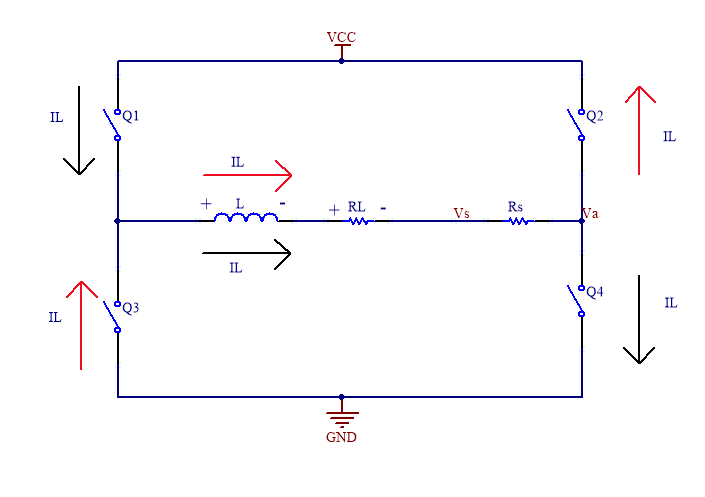
\includegraphics[width=\textwidth]{puente_con_rshunt.png}
	\caption{Puente H con resistencia de sensado de corriente (Rs).}
	\label{fig:img_puente_con_rshunt}
\end{figure}

Por otro lado, la realimentación del controlador de corriente debe ser en forma de tensión, por lo tanto es suficiente con medir la tensión diferencial $V_s-V_a$ y tener en cuenta en el diseño del controlador la ganancia que se tiene al pasar de corriente a tensión.

Aunque este método para medir corriente pareciera directo, presenta algunos inconvenientes en el diseño:

El primero es que al agregar una resistencia en serie al electroimán, se estaría agregando una mayor disipación de potencia en el sistema. Para intentar reducir este problema se podría elegir un valor de resistencia lo suficientemente bajo para que su consumo sea despreciable. Por ejemplo, se podría adoptar una resistencia de $10\:mOhms$. Este valor resulta en pérdidas de potencia de $4\:W$, que es un valor aceptable. 

El segundo inconveniente es que alteraría la dinámica de la planta, ya que la constante de tiempo sería $\tau=\frac{L}{R_L+R_s}$. Sin embargo, el electroimán presenta una resistencia interna de $0.2\:Ohm$, por lo que una resistencia de sensado con valor $10\:mOhm$ no afectaría en gran medida la dinámica.

El tercero es que se debe realizar una medición de tensión flotante. Esto se debe a que la resistencia, al estar en serie con el electroimán, no tiene ningún punto de medición referido a masa. Por lo tanto, se debe utilizar un amplificador que mida tensión en modo diferencial para luego obtener una señal en modo común. El inconveniente que se presenta es que cada uno de los puntos de medición se encuentra a un alto potencial respecto de masa y, además, este cambia en cada conmutación. Esto genera que durante los transitorios de conmutación haya ruido en la medición diferencial.

Debido a que se requiere medir el valor de corriente sin que el ruido de modo común altere la medición, se propone analizar otra alternativa que sea inmune a dicho efecto.


\subsubsection{Análisis de medición de corriente mediante sensor de efecto Hall}

Dado que la medición con una resistencia de sensado introduce ruido ocasionado por la conmutación de las llaves, se plantea la alternativa de utilizar un sensor de efecto Hall. Este dispositivo mide el campo magnético generado por la corriente, entregando a su salida una tensión proporcional a ésta. La principal ventaja que presenta es que el campo magnético medido sólo es sensible a las variaciones de corriente y no a las conmutaciones de tensión.

Existen una gran variedad de estos sensores en el mercado, cada uno con diferentes características. A continuación se mencionan los criterios que se tendrán en cuenta para la elección del sensor:

\begin{itemize}
	\item Debe ser capaz de medir una corriente de hasta $30\:A$.
	\item El ancho de banda debe ser mucho mayor al polo de la frecuencia de conmutación del controlador de corriente para poder conservar la forma de onda de la corriente triangular a medir. Por lo tanto, debe ser al menos de $100\:kHz$.
	\item La transresistencia debe ser lineal entre $0\:A$ y $30\:A$.	
\end{itemize}

A partir de estas características se decidió utilizar el sensor HO 15-NP-0000 \cite{HO15-NP}. Este permite medir una corriente de $\pm 37.5\:A$ con un ancho de banda de $250\:kHz$ y posee una transresistencia de $53.33\:mV/A$ en todo  el rango de corriente. Además, presenta alta inmunidad a interferencias externas. 

Este sensor tiene la capacidad de medir tanto corrientes en sentido positivo, como negativo. Para ello admite una tensión de bias de $2.5\:V$, la cual se corresponde a la salida cuando la corriente es nula. Cuando la circulación de corriente es positiva, la salida del sensor resulta en una tensión mayor a $2.5\:V$, y para negativas, menor.

De esta forma, el bloque H de realimentación queda definido como:

\begin{equation}
	H=\frac{V_iLF}{I_L}=53,33 mV/A
\end{equation}



\subsection{Cálculo de ganancia de entrada}


